\documentclass[11pt,a4paper]{article}
\usepackage{amsmath}
\usepackage{amsfonts}
\usepackage{amssymb}
\usepackage{fancyhdr}
\usepackage{lastpage}
\usepackage{graphicx}
\usepackage{ucs}
\usepackage[utf8x]{inputenc}
\usepackage[italian]{babel}
\usepackage[colorlinks=true,linkcolor=black]{hyperref}

\renewcommand{\headrulewidth}{0.6pt}
\renewcommand{\footrulewidth}{0.6pt}
% impostazione dello stile per le pagine interne del documento
\lhead{\leftmark}
\chead{}
\rhead{
\includegraphics[scale=0.15]{logo.png} }
\lfoot{Specifica tecnica v1.0.0}
\cfoot{}
\rfoot{\thepage \ di \pageref{LastPage}}
% ridefinizione dello stile plain per il frontespizio
\fancypagestyle{plain}{
\fancyhf
}
% impostazione dello stile per l'indice
\fancypagestyle{indice}{
\lhead{\leftmark}
\chead{}
\rhead{
\includegraphics[scale=0.15]{logo.png}}
\lfoot{Specifica tecnica v1.0.0}
\cfoot{}
\rfoot{}
}
\headheight = 46pt
%definizione del comando "\modifiche" per la creazione del diario delle modifiche
\newcommand{\modifiche} 
{
\newpage
\begin{center}
\textbf{Diario delle modifiche} \\
\bigskip
\begin{tabular}{|c|c|p{0.62\textwidth}|}
\hline
\textsc{Data} & \textsc{Versione} & \textsc{Modifica} \\
\hline
\hline
\textit{07-03-2009} & 1.0.0 & Approvazione del responsabile e passaggio di stato a Formale \\
\hline
\textit{11-02-2009} & 0.7.0 & Aggiunta diagramma di sequenza del Middle Man \\
\hline
\textit{10-02-2009} & 0.6.4 & Riscrittura contenuto Middle Man \\
\hline
\textit{24-01-2009} & 0.6.3 & Sottolineatura dei termini del Glossario \\
\hline
\textit{24-01-2009} & 0.6.2 & Correzioni di forma e sintassi \\
\hline
\textit{24-01-2009} & 0.6.1 & Lieve correzione nel diagramma delle classi \\
\hline
\textit{23-01-2009} & 0.6.0 & Aggiunto il tracciamento requisiti-componenti \\
\hline
\textit{22-01-2009} & 0.5.0 & Aggiunta il diagramma e la descrizione delle classi \\
\hline
\textit{21-01-2009} & 0.4.1 & Correzioni varie di tipo ortografico\\
\hline
\textit{21-01-2009} & 0.4.0 & Aggiunto middleman e algorithm \\
\hline
\textit{20-01-2009} & 0.3.1 & Correzioni varie \\
\hline
\textit{20-01-2009} & 0.3.0 & Aggiunti i flussi di esecuzione \\
\hline
\textit{17-01-2009} & 0.2.0 & Stesura Descrizione dei componenti \\
\hline
\textit{15-01-2009} & 0.1.0 & Creazione dell'indice \\
\hline
\end{tabular}
\end{center}
}
%definizione del comando "\info" per la creazione delle informazioni del documento
\newcommand{\info} {
\bigskip
\begin{tabbing}
	\hspace*{0.3\textwidth} \= \hspace*{0.5\textwidth} \kill
	\parbox{0.3\textwidth}{\textbf{Verifica: }} \> \parbox{0.5\textwidth}{Barbiero Mattia} \\
	\parbox{0.3\textwidth}{\textbf{Approvazione: }} \> \parbox{0.5\textwidth}{Freo Matteo} \\
	\parbox{0.3\textwidth}{\textbf{Stato: }} \> \parbox{0.5\textwidth}{Formale} \\
	\parbox{0.3\textwidth}{\textbf{Uso: }} \> \parbox{0.5\textwidth}{Esterno} \\
	\parbox{0.3\textwidth}{\textbf{Distribuzione: }} \> \parbox{0.5\textwidth}{QuiXoft} \\
							\> \parbox{0.5\textwidth}{Rossi Francesca} \\
							\> \parbox{0.5\textwidth}{Vardanega Tullio} \\
							\> \parbox{0.5\textwidth}{Conte Renato} \\
\end{tabbing}
}
%definizione del comando "\frontespizio" per la creazione del frontespizio
\newcommand{\frontespizio} {
\thispagestyle{plain}
\title{\begin{Huge}\textsc{Progetto SIGEOL}\end{Huge} \\ \textit{Specifica Tecnica \\ v1.0.0}}
\author{Redazione: Grosselle Alessandro, Scarpa Davide}
\maketitle
\medskip
\begin{center}

\includegraphics[scale=0.5]{logo.png} \\
\textit{quixoft.sol@gmail.com}
\end{center}
\medskip
\info
\begin{center}
\textbf{Sommario} \\
Documento contenente la descrizione dettaglia dei componenti presenti nel sistema ''SIGEOL'' commissionato dalla prof. Rossi Francesca.
\end{center}
\newpage
}
%definizione del comando "\indice" per la creazione dell'indice
\newcommand{\indice} {
\thispagestyle{indice}
\tableofcontents
\newpage
}
\pagestyle{fancy}
\begin{document}
\frontespizio
\indice
\setcounter{page}{1}
\section{Introduzione}
\subsection{Scopo del documento}
Il presente documento denominato \textsc{Specifica tecnica} ha lo scopo di mostra\-re la struttura del progetto \textit{SIGEOL} e descrivere i componenti che ne fanno parte. 
\subsection{Scopo del prodotto}
Il progetto sotto analisi, denominato \textit{SIGEOL}, si prefigge di automatizzare la generazione, la gestione, l'ottimizzazione e la consultazione degli orari di lezione. Per maggiori dettagli consultare il documento denominato \textsc{Analisi dei Requisiti} alla sua ultima versione.
\subsection{Glossario}
Le definizioni dei termini specialistici usati nella stesura di questo e di tutti gli altri documenti possono essere trovate nel documento \textsc{Glossario} al fine di eliminare ogni ambiguità e di facilitare la comprensione dei temi trattati. Ogni termine la cui definizione è disponibile all’interno del Glossario verrà marcato con una \underline{sottolineatura}.

\section{Definizione del prodotto}
\subsection{Metodo e formalismo di specifica}
Lo strumento principale nel redarre la specifica tecnica sarà il linguaggio \underline{UML}, che permetterà di realizzare i diagrammi delle classi, di sequenza, di collaborazione e di attività.


La decomposizione architetturale utilizzata sarà di tipo \underline{Top-down}.
E' prevista una descrizione generale dell’architettura del sistema, alla quale seguiranno le specifiche dettagliate dei suoi componenti.


Per semplificare la progettazione, si utilizzeranno i seguenti \underline{pattern}:
\begin{description}
 \item[\textbf{MVC}] 
Il \underline{pattern} MVC (Model View Controller) si basa sulla separazione tra i componenti software del sistema, che gestiscono il modo in cui presentare i dati, e i componenti che gestiscono i dati stessi. 
 \item[\textbf{Façade}]
Permette, attraverso un'interfaccia più semplice, l'accesso a sottosistemi aventi interfacce complesse e molto diverse tra loro, nonché a blocchi di codice complessi.
\item[\textbf{REST}]
Representational state transfer (REST) è un tipo di architettura software per i sistemi di ipertesto distribuiti come il World Wide Web. 
REST si riferisce ad un insieme di principi di architetture di rete, i quali delineano come le risorse sono definite e indirizzate.


\item[\textbf{Convention Over Configuration}]
Convention Over Configuration è un paradigma di programmazione che prevede configurazione minima (o addirittura assente) per il programmatore che utilizza un \underline{framework} che lo rispetti, obbligandolo a configurare solo gli aspetti che si differenziano dalle implementazioni standard o che non rispettano particolari convenzioni di denominazione o simili.
Significa che Rails prevede delle impostazioni di default per qualsiasi aspetto dell’applicazione. Utilizzando queste convenzioni sarà possibile velocizzare i tempi di sviluppo evitando di realizzare scomodi file di configurazione. L’esempio più chiaro del COC si può notare a livello di modelli: rispettando le convenzioni previste dal \underline{framework} è possibile realizzare strutture di dati complesse con molte relazioni tra oggetti in pochissimo tempo, in maniera quasi meccanica e soprattutto senza definire nessuna configurazione. Questo concetto differenzia Rails dai \underline{framework} che prevedono molte righe di configurazione per ogni aspetto dell’applicazione. Con il COC tutto diventa più snello e più dinamico. Ovviamente per situazioni in cui le convenzioni non possano essere rispettate, Rails permette di utilizzare schemi funzionali diversi da quelli previsti.
\item[\textbf{DRY}]
Questo concetto, fortemente filosofico, prevede che ciascun elemento di un’applicazione debba essere implementato solamente una volta e niente debba essere ripetuto. Questo significa che, mediante Rails, è possibile gestire funzionalità ripetitive con una estrema fattorizzazione del codice (''scrivo una volta e uso più volte'') che facilita sia lo sviluppo iniziale che eventuali modifiche successive del prodotto.
\item[\textbf{View Helper}]
Questo \underline{pattern} disaccoppia il Business Logic dallo strato View, il che facilita
la manutenibilità. Aiuta a separare, in fase di sviluppo, la responsabilità
del web designer e dello sviluppatore.
\item[\textbf{Active Record}]
Secondo il \underline{pattern} Active Record esiste una relazione molto stretta fra tabella e classe, colonne e attributi della classe. 
\begin{itemize}
 \item una tabella di un \underline{database} relazionale è gestita attraverso una classe
\item una singola istanza della classe corrisponde ad una riga della tabella
\item alla creazione di una nuova istanza viene creata una nuova riga all'interno della tabella, e modificando l'istanza la riga viene aggiornata
\end{itemize}
\end{description}


Il sistema verrà implementato utilizzando \underline{Ruby on Rails}, un \underline{framework} la cui architettura è fortemente ispirata al paradigma Model-View-Controller. 
Oltre a veicolare lo sviluppo di applicazioni secondo il \underline{pattern} MVC, Rails segui la filosofia REST imponendo un’ulteriore disciplina nella codifica degli indirizzi garantendo quindi maggior chiarezza e compattezza.


\subsection{Presentazione dell'architettura generale del sistema}
Per presentare l'architettura generale del sistema \textit{Sigeol} si utilizzerà il \underline{pattern} Model-View-Controller(MVC).
In questo modello i ruoli di presentazione, controllo ed accesso ai dati vengono affidati a componenti diversi e sono tra di loro disaccoppiati.

Sono inoltre previste altre due componenti: Middle Man si occupa di ricevere i compiti che necessitano di un elevato carico di lavoro; Algorithm, invece, risolve il problema del calcolo dell'orario.
\begin{center}
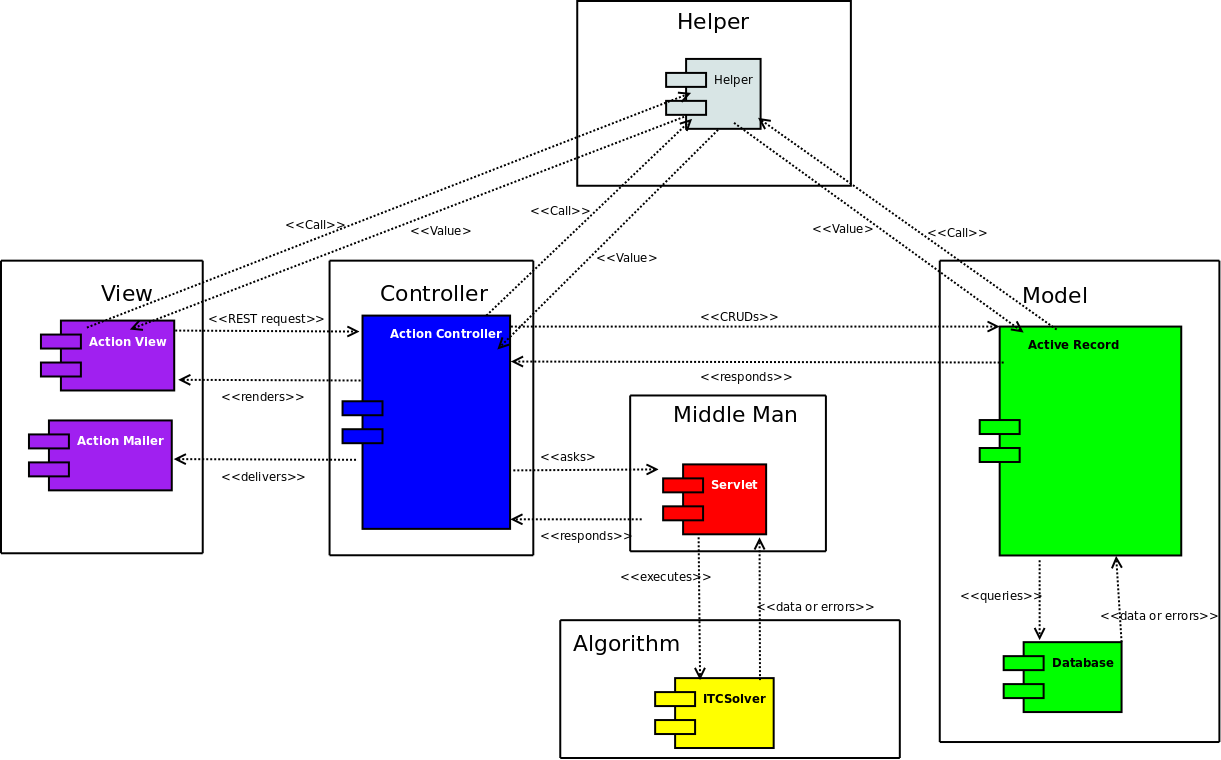
\includegraphics[scale=0.2]{images/component_diagram.png}
\end{center}

\section{Descrizione dei singoli componenti}
\subsection{Model}
L' ActiveRecord è il modulo di \underline{Ruby on Rails} che gestisce la persistenza dei dati. 
Il modulo è stato implementato seguendo il \underline{pattern} Active Record facendo largo uso di convenzioni sui nomi da assegnare a tabelle, classi, colonne e attributi; se non sono presenti configurazioni particolari del modello, sono valide le seguenti convenzioni:
\begin{itemize}
 \item per ogni modello esiste una tabella avente come nome il nome del modello al plurale e in caratteri minuscoli;
\item nel caso di modelli con nome composto di più parole, il nome del modello ha la prima lettera di ogni parola; maiuscola, mentre la tabella ha sempre il nome tutto in minuscolo e separa le parole con un trattino basso (underscore);
\item per ogni colonna della tabella viene reso disponibile il relativo attributo con lo stesso nome;
\item ogni tabella ha una colonna id (intero positivo) che identifica univocamente ogni record;
\end{itemize}
La classe è descritta in buona parte dalla tabella che rappresenta ed espone i metodi necessari per leggere e scrivere i record.
Con ActiveRecord è possibile utilizzare diversi tipi di \underline{database}: SQLite, MySQL, Postgresql, Oracle, IBM DB/2 ed è possibile scrivere driver personalizzati per altri \underline{database} relazionali.
\subsubsection{Relazione d'uso con le altre componenti}
Questa componente si relaziona con il Controller fornendo i dati che vengono richiesti e salvando le eventuali modifiche al \underline{database}.
\subsection{Controller}
Il modulo che gestisce la parte controller è contenuto all'interno del \underline{framework} \underline{Ruby on Rails} ed è chiamato Action Controller.
Questo, assieme all'Action View(confronta sezione \ref{view}) è integrato all'interno di un pacchetto chiamato Action Pack.

Ogni controller è una normale classe, ed ogni metodo pubblico definito in questa classe corrisponde ad un'azione specifica.


\underline{Ruby on Rails} riconosce il tipo di richiesta pervenuta codificando le informazioni all'interno di un URL e si serve di un componente chiamato Rounting, per determinare l'azione cui deve essere sottoposta la richiesta.
Il componente Routing traccia una mappatura che permette a Rails di collegare gli URL esterni e l'azione contenuta in una determinata classe Controller.

Ad esempio, dato un URL nel formato \textit{controller/azione/id}, viene identificato il Controller \textit{controller} e viene istanziato. A questo punto l'oggetto richiama il metodo con nome \textit{azione} e con parametro \textit{id}. Il Controller infine cercherà di visualizzare un \underline{template} con lo stesso nome dell'azione. 
\subsubsection{Relazione d'uso con le altre componenti}
Questa componente si relazione con la View, il Model ed il Middle Man. 

Il Controller funge da intermediario fornendo i dati alla View attraverso il Model. Inoltre sceglie quale view renderizzare a seconda della richiesta pervenuta.

\subsection{View}\label{view}
 Il modulo Action View contenuto nel \underline{framework} \underline{Ruby on Rails}, offre meccanismi avanzati per il riutilizzo del codice, tramite l'uso di viste, \underline{layouts}, partials e di metodi helper pensati per generare ad esempio pagine \underline{XHTML}.
I metodi helper sono semplici metodi pubblici di una classe Controller.
\subsubsection{Relazione d'uso con le altre componenti}
Questa componente si trova in relazione solamente con il Controller. Converte infatti le azioni che l'utente effettua attraverso la View in richieste a metodi propri del Controller.
\subsection{Middle Man}
La componente Middle Man è estranea al \underline{pattern} MVC e si occupa di gestire quelle richieste che a causa del tempo di calcolo, renderebbero inutilizzabile ogni altra funzione di consultazione dell'applicazione web. 
Questa componente sarà implementata tramite una \underline{servlet} in \underline{Java} denominata SchedulerServlet.
La componente integrerà Quartz (un' open source job scheduling system, per maggiori informazioni visitare \\ http://www.opensymphony.com/quartz/ ) il quale verrà utilizzato per gestire tutte le operazioni di scheduling e fornirà strumenti aggiuntivi (quali ripristino informazioni dopo crash di sistema e gestione schedulazioni in formato cron).
\subsubsection{Relazione d'uso con le altre componenti}
Questa componente è in relazione con il Controller e l'Algorithm. 

Per soddifare le richieste del Controller preleva i dati necessari da un file, creato dall'applicazione stessa, e si occuperà poi di avviare la componente Algorithm per il calcolo degli orari passandogli tutti i dati necessari.
Inoltre la componente è utilizzata dal Controller per l'inserimento delle tempistiche di esecuzione del calcolo degli orari.

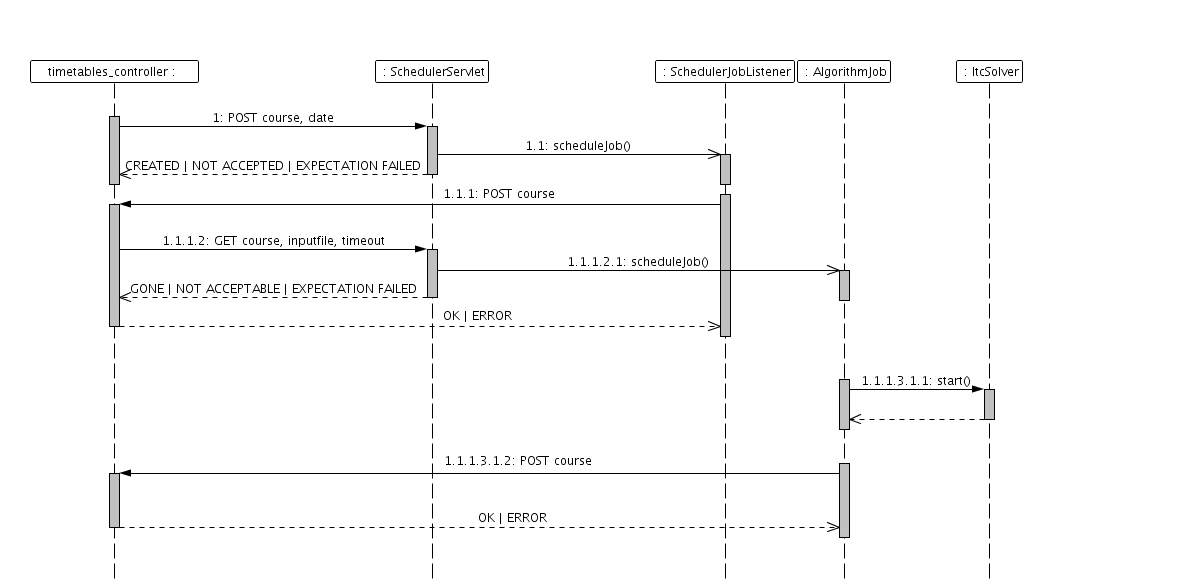
\includegraphics[scale=0.3]{images/MiddleMan_sequence_diagram.png}
% MiddleMan_sequence_diagram.png: 1364x579 pixel, 72dpi, 48.12x20.43 cm, bb=0 0 1364 579
\begin{itemize}
\item 1: impostazione di una nuova generazione dell'orario di un corso di laurea ad una specifica data
\item 1.1: impostazione della classe da istanziare all'avvio dell'evento schedulato
\item 1.1.1: invio della notifica all'applicazione per la preparazione file di input e avvio calcolo
\item 1.1.1.2: invio dei dati alla servlet utili alla generazione dell'orario (manuale e schedulata)
\item 1.1.1.2.1: impostazione dell'istanza di classe che si occuperà di avviare l'algoritmo
\item 1.1.1.3.1.1: avvio dell'algoritmo
\item 1.1.1.3.1.2: segnalazione della generazione dell'orario effettuata (o di eventuale errore)	
\end{itemize}

\subsection{Algorithm}
La componente Algorithm non inclusa nel \underline{pattern} MVC si occupa di calcolare effettivamente l'orario delle lezioni, rispettando i vincoli inseriti nel sistema. Dagli studi di ricerca operativa sono noti diversi algoritmi per la ricerca di una soluzione ottimale di un problema sottoposto a vincoli. L'algoritmo scelto è stato utilizzato nell'International Timetabling Competition 2007 ed è basato sulla libreria Constraint Solver Library (licenza GNU LGPL).
\subsection{Relazioni d'uso di altre componenti}
Questa componente si trova in relazione solo con la componente Middle Man. Algorithm restituisce il risultato in un file che verrà poi processato dall'applicazione.

\section{Diagrammi delle classi}
\subsection{Model}
Rails preferisce le convenzioni alle configurazioni, e cerca di evitare allo sviluppatore il peso di dover specificare l'associazione tra tabelle e classi.
Non è quindi necessario illustrare nella specifica tecnica la struttura del database, in quanto verrà implementato da Rails a partire dalla struttura delle classi.

L'utilizzo dell'inglese nella scelta dei nomi delle classi è necessario per rispettare le convenzioni di Rails.
I nomi delle tabelle del database di sistema saranno semplicemente il plurale dei nomi delle classi qui di seguito specificate:
\\
\begin{center}
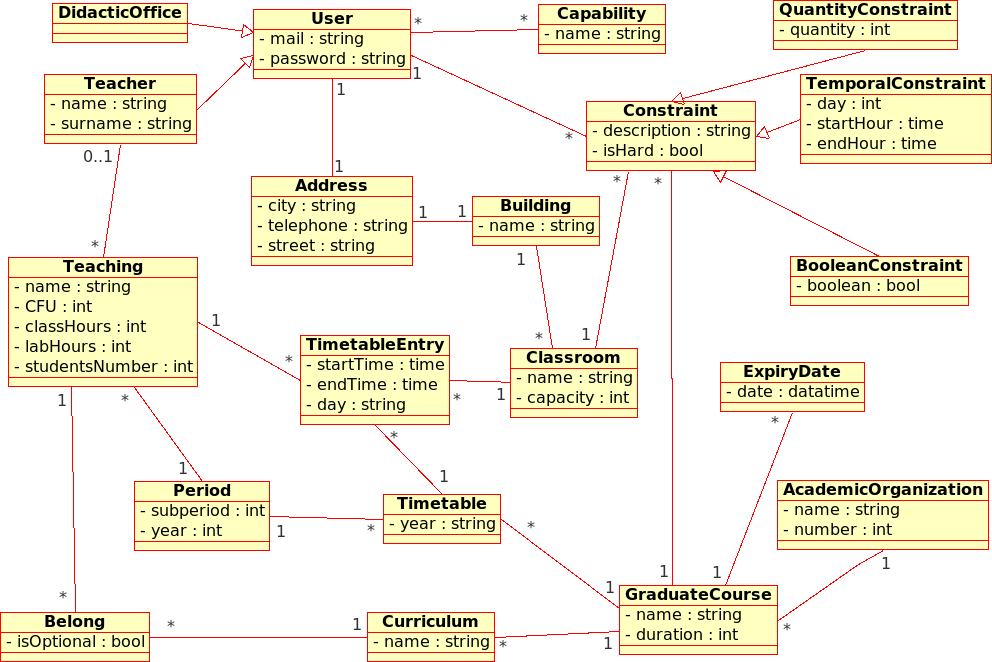
\includegraphics[scale=0.33]{images/class_diagram.png}
\end{center}

\begin{itemize}
\item \textbf{Address}: rappresenta la classe che individua un indirizzo civico.

\item \textbf{Belong}: rappresenta la classe che individua se un determinato insegnamento, inserito in un preciso corso di laurea, e' opzionale o meno.

\item \textbf{Building}: rappresenta la classe che gestisce i dati di un complesso. Quest'ultimo possiede aule, laboratori e uffici dei docenti.

\item \textbf{Capability}: rappresenta la classe che gestisce le informazioni di un determinato servizio, disponibile per gli utenti del sistema. Ogni tipologia di utente ha uno specifico numero di servizi a sua disposizione.

\item \textbf{Constraint}: rappresenta la classe che individua un vincolo o una preferenza, necessario/a al calcolo dello schema d'orario. L'attributo booleano isHard indica se è un vincolo o una preferenza.
\subitem \textbf{QuantityConstraint}: rappresenta la classe che individua un vincolo di tipo numerico; ad esempio il numero massimo di ore di una lezione. La classe QuantityConstraint è in associazione polimorfa con la classe Constraint.
\subitem \textbf{TemporalConstraint}: rappresenta la classe che individua un vincolo di tipo temporale, specificato da un giorno della settimana, un'ora di inizio ed un'ora di fine. La classe TemporalConstraint è in associazione polimorfa con la classe Constraint.
\subitem \textbf{BooleanConstraint}: rappresenta la classe che individua un vincolo che potrà essere considerato o meno dall'algoritmo in base al valore del suo attributo booleano. La classe BooleanConstraint è in associazione polimorfa con la classe Constraint.

\item \textbf{Curriculum}: rappresenta la classe che individua un percorso formativo appartenetente ad un corso di laurea.

\item \textbf{ExpiryDate}: rappresenta la classe che individua la data oltre la quale un docente non potrà più inserire e/o modificare i propri vincoli e preferenze. Successivamente a questa data l'algoritmo di calcolo dello schema d'orario si avvierà. 

\item \textbf{GraduateCourse}: rappresenta la classe che individua un corso di laurea e ne gestisce i relativi dati.

\item \textbf{AcademicOrganization}: rappresenta la classe che descrive com'è strutturato un corso di laurea: bimestre, trimestre, semestre.

\item \textbf{Period}: rappresenta la classe che individua una fascia temporale.
Le fascie temporali sono generate in base alla durata e alla struttura del corso di laurea (bimestre, trimestre, semestre). Ogni insegnamento è inserito in una specifica fascia temporale; ad esempio primo (year) anno, primo (subperiod) trimestre.

\item \textbf{Teaching}: rappresenta la classe che gestisce i dati relativi ad un determinato insegnamento.

\item \textbf{Timetable}: rappresenta la classe che permette di individuare lo schema d'orario specifico di un corso di laurea e di un periodo (bimestre, trimestre, semestre) 

\item \textbf{TimetableEntry}: rappresenta la classe che individua un giorno, un'ora di inizio e un'ora di fine di un determinato insegnamento.

\item \textbf{User}: rappresenta la classe che gestisce i dati di \underline{login}. In particolare possiede i seguenti due attributi: mail (che funge da username) e password (che permette l'\underline{autenticazione} sicura).
\subitem \textbf{DidacticOffice}: rappresenta la classe che gestisce i dati della segreteria. 
Questa classe e' in associazione polimorfa con la classe User 
\subitem \textbf{Teacher}: rappresenta la classe che gestisce i dati personali di un docente.
Questa classe e' in associazione polimorfa con la classe User. 
\end{itemize}
\section{Flusso di esecuzione}
La seguente sezione si fa carico di illustrare, con l'utilizzo di diagrammi di attività, i flussi delle varie azioni che gli utenti del sistema SIGEOL hanno la possibilità di compiere.
Quanto riportato in seguito è da considerarsi passibile di modifiche col procedere della fase di progettazione.
\newpage
\subsection{Login utenti}
La Segreteria Didattica e tutti Docenti registrati hanno la possibilità di accedere alla pagina di \underline{login} per inserire le proprie credenziali ed accedere alle funzioni aggiuntive che il sistema SIGEOL mette loro a disposizione. Il Presidente del CCS viene considerato un Docente, ma con in più la possibilità di accedere a tutte le funzioni tipiche della Segreteria Didattica.

Al termine della fase di \underline{login}, l'utente verrà reindirizzato alla pagina principale di SIGEOL e potrà espletare le funzioni a sua disposizione.\\
\begin{center}
 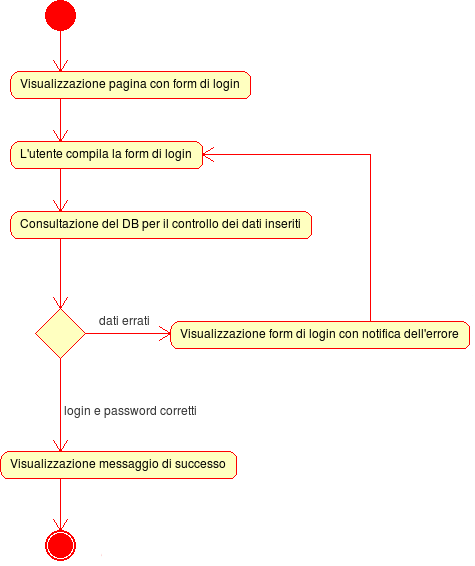
\includegraphics[scale=1]{images/login.png}
\end{center}

\newpage
\subsection{Inserimento nuovo Docente}
La Segreteria Didattica e il Presidente del CCS hanno la possibilità, dopo aver effettuato con successo il \underline{login}, di inserire un nuovo Docente nel sistema SIGEOL. Verranno richiesti nome, cognome ed indirizzo email. Se tali dati vengono inseriti e il Docente non è già presente nel DB di sistema, viene automaticamente inviata una email al Docente invitato, in cui gli viene indicato il \underline{link} necessario per procedere alla creazione del suo \underline{account}.\\
\begin{center}
 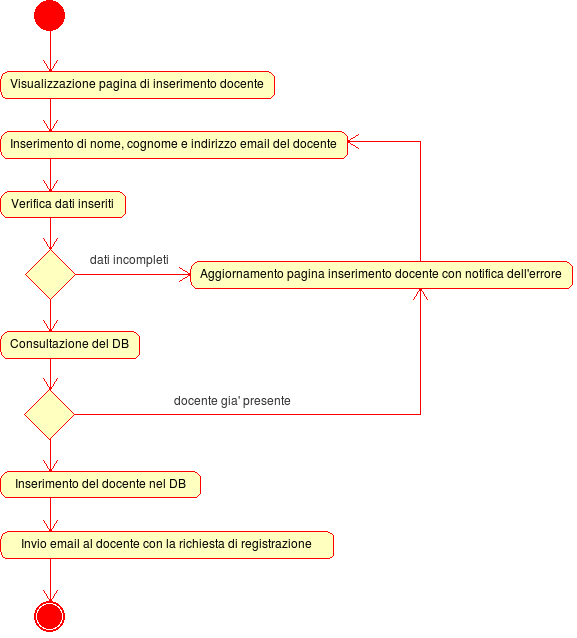
\includegraphics[scale=0.9]{images/inserimento_docente.png}
\end{center}

\newpage
\subsection{Registrazione Docente}
Ogni docente, dopo aver ricevuto la mail di invito al sistema SIGEOL, utilizza il \underline{link} ricevuto per accedere al form di scelta password e di inserimento degli altri dati personali. La scelta della password seguirà rigide regole di sintassi, che verranno controllate dinamicamente durante l'inserimento. Tali regole prevederanno un numero minimo di caratteri, la presenza obbligatoria di cifre o simboli e altre convenzioni che saranno decise dal team QuiXoft, in collaborazione con il Committente, durante il proseguimento della fase di progettazione. La password dovrà poi essere confermata in un successivo campo dati, per evitare spiacevoli errori di battitura.

Al termine della prcedura la password scelta e gli altri dati inseriti verranno memorizzati in modo sicuro sul DB di sistema. \\
\begin{center}
 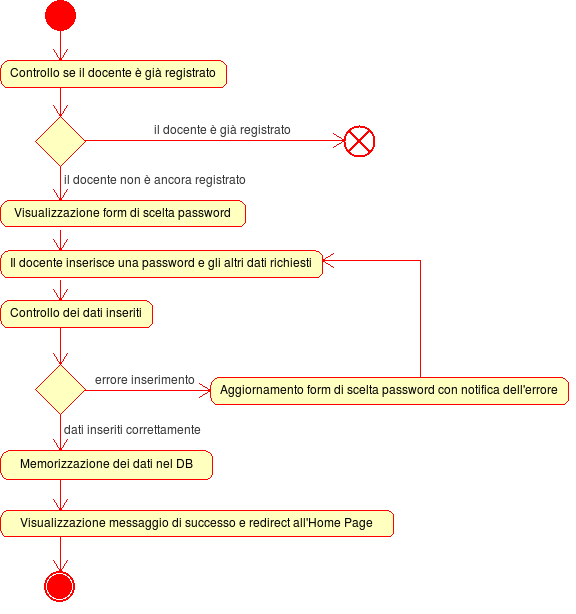
\includegraphics[scale=0.8]{images/registrazione_docente.png}
\end{center}

\newpage
\subsection{Inserimento dei dati nel sistema}
La Segreteria Didattica e il Presidente del CCS hanno la possibilità di inserire i dati relativi ai corsi di laurea, agli insegnamenti, alle aule, ai dipartimenti e molti altri dati indispensabili al funzionamento del sistema SIGEOL.

L'inserimento avverrà tramite diverse pagine web e diverse form, ma il diagramma di flusso di tali inserimenti è cosi simile che è stato scelto di esporne solo uno generale, adatto a rappresentare tutti gli inserimenti. \\
\begin{center}
 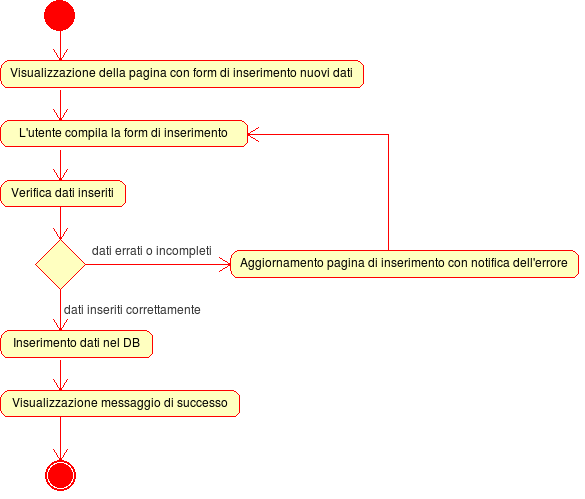
\includegraphics[scale=0.85]{images/inserimento_dati.png}
\end{center}

\newpage
\subsection{Modifica dei dati del sistema}
La Segreteria Didattica e il Presidente del CCS hanno la possibilità di modificare tutti i dati relativi ai corsi di laurea, agli insegnamenti, alle aule, ai dipartimenti, ecc...

I docenti invece hanno la possibilità di modificare i propri dati personali e i vincoli e le preferenze inserite.

Le similitudini tra tutte le sopra citate modifiche hanno portato allo sviluppo di un singolo diagramma di attività che le rappresenti tutte. L'invocazione del comando di modifica sarà ovviamente diverso tra i vari tipi di dati, ma la procedura per modificarli e salvarli è similare.
\begin{center}
 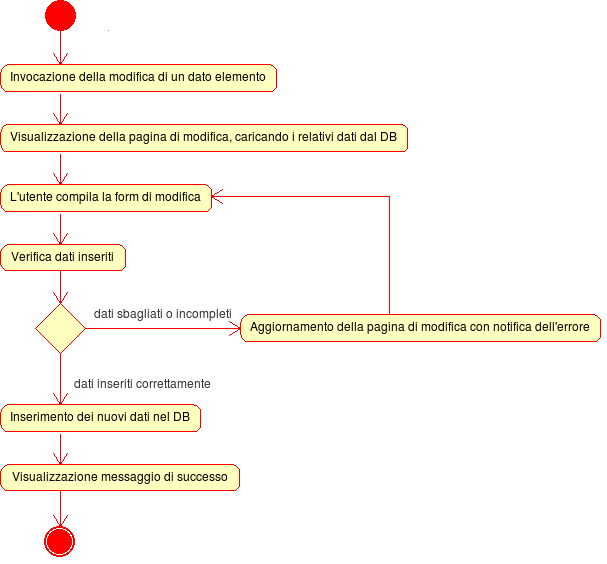
\includegraphics[scale=0.85]{images/modifica_dati.png}
\end{center}

\newpage
\subsection{Inserimento vincoli e preferenze da parte dei Docenti}
Tutti i docenti cha abbiano effettuato correttamente il \underline{login} hanno la possibilità di inserire i loro vincoli e le loro preferenze. La procedura è similare, per tanto è rappresentata dallo stesso diagramma di attività.

La differenza sostanziale nell'inserimento di un vincolo o di una preferenza è che solo il vincolo, tra i due, prevede una motivazione, mentre solo la preferenza prevede un livello di priorità. L'assegnazione della priorità di una preferenza è automatizzata dal sistema: il Docente dovrà solamente decidere l'ordine di importanza delle proprie preferenze.
\begin{center}
 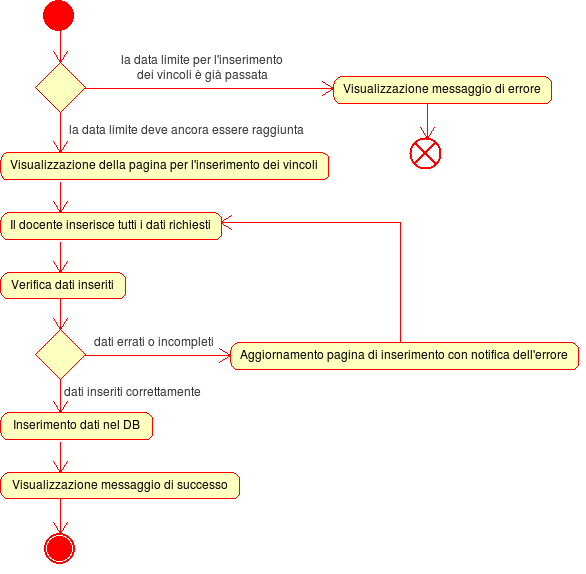
\includegraphics[scale=0.85]{images/inserimento_vincoli.png}
\end{center}
\newpage
\subsection{Generazione dell'orario}
La Segreteria Didattica e il Presidente del CCS hanno la possibilità, una volta scaduta la data limite per l'inserimento dei vincoli e delle preferenze da parte dei Docenti, di far partire l'algoritmo di generazione dell'orario. L'algoritmo calcolerà l'orario migliore possibile per tutti i Corsi di Laurea inseriti, e sarà data la possibilità di scelta se generare l'orario per uno o più periodi (per periodo si intende il numero di trimestre-semestre-ecc... in base alla scelta fatta nel momento di inserimento dei dati).

L'algoritmo proporrà un orario soddisfacendo tutti i requisiti presenti e tentando di rispettare il più possibile tutte le preferenze. Se ciò non fosse possibile, sarà data la possibilità alla Segreteria Didattica o al Presidente del CCS di rilassare certi vincoli o di modificare manualmente lo schema d'orario generato.
\begin{center}
 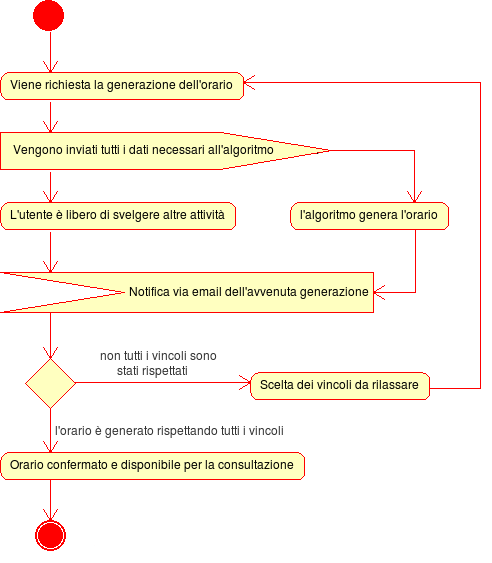
\includegraphics[scale=0.85]{images/generazione_orario.png}
\end{center}
\newpage
\subsection{Consultazione dell'orario}
Qualsiasi utente ha la possibilità di consultare gli orari generati dal sistema SIGEOL, anche senza effettuare alcuna operazione di \underline{login}. Sarà sufficiente scegliere il Corso di Laurea ed il periodo e verrà visualizzato il relativo orario.

Cliccando su un determinato insegnamento sarà possibile consultarne le informazioni.
Quest'operazione può essere compiuta quante volte si vuole, senza modificare la visualizzazione dell'orario: le informazioni saranno infatti mostrate su una nuova pagina o su una finestra pop-up. Con il proseguire della fase di progettazione verrà definitivamente decisa la forma di visualizzazione.

In ogni momento è data la possibilità all'utente di generare un \underline{PDF} contenente l'orario visualizzato: sarà possibili visualizzarlo all'interno del proprio \underline{browser} oppure salvarlo.
\begin{center}
 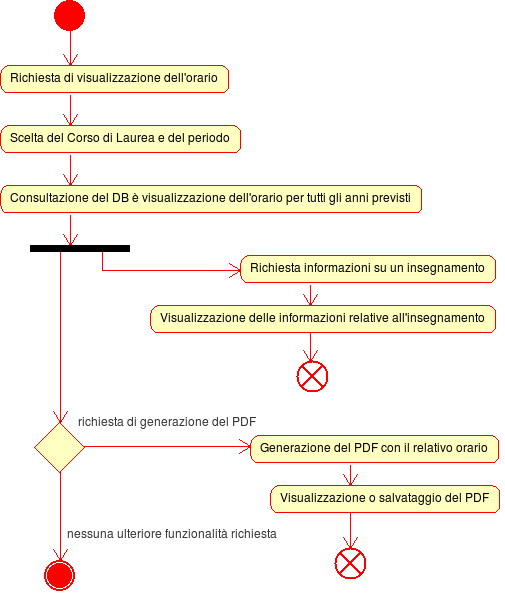
\includegraphics[scale=0.85]{images/consultazione_orario.png}
\end{center}
\section{Tracciamento componenti-requisiti}
Di seguito è riportato il tracciamento dei requisiti descritti nel documento denominato \textsc{Analisi dei Requisiti} con le componenti descritti nel presente.\\
\begin{center}
\begin{small}
\begin{tabular}{|c||c|c|c|c|c|}
\hline
\textsc{Requisiti} & \textsc{View} & \textsc{Controller} & \textsc{Model} & \textsc{MiddleMan} & \textsc{Algorithm}\\ \hline \hline
RFO0.0 & \checkmark & \checkmark & \checkmark & & \\
\hline
RFO0.1 & \checkmark & \checkmark & \checkmark & & \\
\hline
RFO0.2 & \checkmark & \checkmark & \checkmark & & \\
\hline
RFO0.3 & \checkmark & \checkmark & \checkmark & & \\
\hline
RFO0.4 & \checkmark & \checkmark & \checkmark & & \\
\hline
RFO0.5 & \checkmark & \checkmark & \checkmark & & \\
\hline
RFO0.6 & \checkmark & \checkmark & \checkmark & & \\
\hline
RFO0.7 & \checkmark & \checkmark & \checkmark & \checkmark & \checkmark \\
\hline
RFO0.8 & \checkmark & \checkmark & \checkmark & & \\
\hline
RFO0.9 & \checkmark & \checkmark & \checkmark & & \\
\hline
RFO0.10 & \checkmark & \checkmark & \checkmark & & \\
\hline
RFO0.11 & \checkmark & \checkmark & \checkmark & & \\
\hline
RFO0.12 & \checkmark & \checkmark & \checkmark & & \\
\hline
RFO0.13 & \checkmark & \checkmark & \checkmark & & \\
\hline
RFO0.14 & \checkmark & \checkmark & \checkmark & & \\
\hline
RFO0.15 & \checkmark & \checkmark & \checkmark & & \\
\hline
RFO0.16 & \checkmark & \checkmark & \checkmark & & \\
\hline
RFO0.17 & \checkmark & \checkmark & \checkmark & & \\
\hline
RFO0.18 & \checkmark & \checkmark & \checkmark & & \\
\hline
RFO0.19 & \checkmark & \checkmark & \checkmark & & \\
\hline
RFO0.20 & \checkmark & \checkmark & \checkmark & & \\
\hline
RFO0.21 & \checkmark & \checkmark & \checkmark & & \\
\hline
RFO0.22 & \checkmark & \checkmark & \checkmark & & \\
\hline
RFO0.23 & \checkmark & \checkmark & \checkmark & & \\
\hline
RFO0.24 & \checkmark & \checkmark & \checkmark & & \\
\hline
\end{tabular}
\end{small}
\end{center}
\begin{center}
\begin{small}
\begin{tabular}{|c||c|c|c|c|c|}
\hline
\textsc{Requisiti} & \textsc{View} & \textsc{Controller} & \textsc{Model} & \textsc{MiddleMan} & \textsc{Algorithm}\\ \hline \hline
RFO1.0 & \checkmark & \checkmark & \checkmark & & \\
\hline
RFO1.1 & \checkmark & \checkmark & \checkmark & & \\
\hline
RFO1.2 & \checkmark & \checkmark & \checkmark & & \\
\hline
RFO1.3 & \checkmark & \checkmark & \checkmark & & \\
\hline
RFO1.4 & \checkmark & \checkmark & \checkmark & & \\
\hline
RFO1.5 & \checkmark & \checkmark & \checkmark & & \\
\hline
RFO1.6 & \checkmark & \checkmark & \checkmark & & \\
\hline
RFD0.0 & \checkmark & \checkmark & \checkmark & & \\
\hline
RFD0.1 & \checkmark & \checkmark & \checkmark & & \\
\hline
RFD0.2 & & & \checkmark & \checkmark & \\
\hline
RFD0.3 & \checkmark & \checkmark & \checkmark & & \\
\hline
RFD1.0 & \checkmark & \checkmark & \checkmark & & \\
\hline
RFD2.0 & \checkmark & \checkmark & \checkmark & & \\
\hline
RFD2.1 & \checkmark & \checkmark & \checkmark & & \\
\hline
RQO0 & \checkmark & & & & \\
\hline
RQO1 & & & \checkmark & & \\
\hline
RQO2 & & \checkmark & \checkmark & & \\
\hline
RQO3 & \checkmark & \checkmark & \checkmark & \checkmark & \checkmark \\
\hline
RQO4 & \checkmark & & & & \\
\hline
RQO5 & \checkmark & & & & \\
\hline
RQO6 & \checkmark & \checkmark & \checkmark & \checkmark & \checkmark \\
\hline
RQD1 & & \checkmark & \checkmark & & \\
\hline
RIO0.0 & & & \checkmark & & \\
\hline
RIO1.0 & \checkmark & \checkmark & \checkmark & & \\
\hline
RIO1.1 & \checkmark & \checkmark & \checkmark & & \\
\hline
RIO1.2 & \checkmark & & & & \\
\hline
RID0.0 & \checkmark & \checkmark & \checkmark & \checkmark & \checkmark \\
\hline
\end{tabular}
\end{small}
\end{center}
\medskip

\modifiche
\end{document}
